\documentclass[a4paper,11pt]{article}
\usepackage{graphicx}
\usepackage{booktabs}
\usepackage{setspace}
\usepackage{parskip}
\usepackage[english]{babel}
\usepackage{refstyle}
\usepackage{hyperref}
\usepackage{caption}
\usepackage{subcaption}
\usepackage{amsmath}
\usepackage{amssymb} %Pfeilbefehle
\usepackage{dsfont}

\onehalfspacing
\begin{document}
\author{Mario Tambos}
\title{\vspace{-2cm}Report for Sheet 04\\
\small{Lab Course Machine Learning and Data Analysis}}
\maketitle

\section*{Implementation comments}

The code was structured mostly in functions following an imperative paradigm, except for the \verb|svm_smo| and \verb|svm_qp| classes, which were required by the assignment's statement, and the ancillary \verb|SupervisedMethod| class.

One function was declared for each assignment in Part 2.

Beyond \verb|matplotlib|, \verb|numpy| and \verb|scipy|, \verb|seaborn| was used to improve the plots aesthetics in Part 2, \verb|scikit-learn| for hyperparameter selection and \verb|joblib| to parallellize some tasks.


All tasks were completed, and all tests passed.

For some, as of the time of this writing, undiscovered reason, the \verb|cv| function written (included in the code for reference) did not work as expected.
Therefore, \verb|scikit-learn|'s \verb|GridSearchCV| was used for the experiments in Part 2.

Moreover, using the written \verb|svm_smo| class in Assignment 7 caused an extremely long run time (unfinished after more than 10 hours, see \verb|assignment7_own| function).
Consequently, \verb|scikit-learn|'s \verb|SVC| class was used instead for this experiment.
 
In all experiments, the \verb|zero-one-loss| functions was chosen as the objective to minimize.

\section*{Assignment 3}

If we set the variables as follows:

\begin{align*}
    P_{i,j} &= y_i * y_j * k(x_i, x_j); \vec{P}\in \mathbb{R}^{n\times n} \\
    \vec{q} &= -\mathds{1};\quad \vec{q} \in \mathbb{R}^n \\
    G_{i,j} &= -\mathbb{I}; \quad \vec{G}\in\mathbb{R}^{n\times n}\\
    \vec{h} &= \vec{0};\quad \vec{h} \in \mathbb{R}^{n} \\
    A_{1,i} &= y_i; \quad \vec{A} \in \mathbb{R}^{1\times n}\\
    b &= 0;\quad b \in \mathbb{R}
\end{align*}

and considering that $\max_{x} f(x) = \min_{x} -f(x)$, then the \verb|cvxopt| quadratic optimization problem is equivalent to the dual of the SVM problem. In the \verb|cvxopt| formulation, the variable $\vec{x}$ corresponds to the $\vec{\alpha}$ of the SVM dual.

\section*{Assignment 4}
\subsection*{Point 1.}

\Figref{assignment4_1} shows the decision boundary of the model trained with the best $C$ and $\sigma$ parameters, found using cross validated grid search.

\begin{figure}
    \centering
    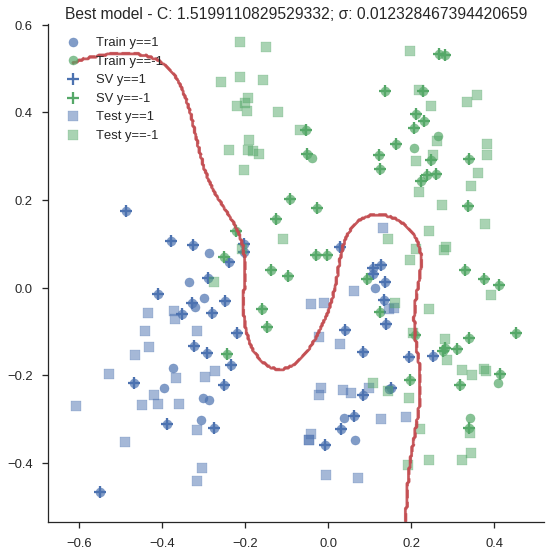
\includegraphics[width=0.7\textwidth]{images/assignment4_1.png}
    \caption{Scatter plot of the \texttt{easy\_2d} dataset, and decision boundary for the SVM's optimal $C$ and $\sigma$ parameters.}
    \label{fig:assignment4_1}
\end{figure}

\subsection*{Point 2.}

\Figref{assignment4_2} shows the decision boundaries of under- and over-fitting SVM models.
For the under-fitting model $C=100$ and $\sigma=100$ were used.
For the over-fitting model $C=1$ and $\sigma=0.001$ were used.

\begin{figure}
    \centering
    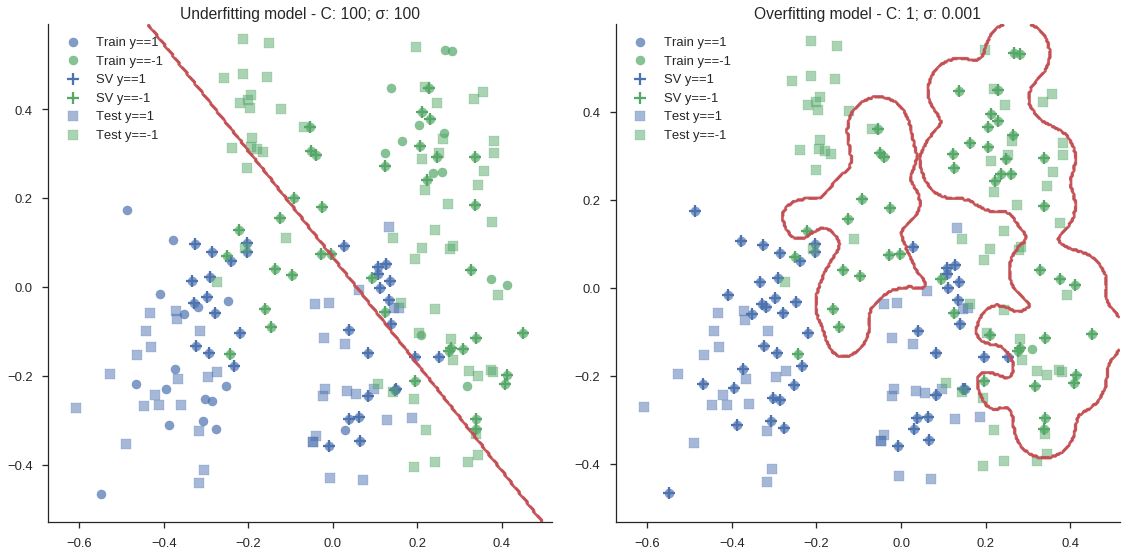
\includegraphics[width=\textwidth]{images/assignment4_2.png}
    \caption{Scatter plots of the \texttt{easy\_2d} dataset, and decision boundaries for under- (left) and over-fitting (right) SVMs.}
    \label{fig:assignment4_2}
\end{figure}

\subsection*{Point 3.}

\Figref{assignment4_3} shows the ROC curve resulting from varying the $b$ parameter in the model from Point 1.
The model's parameters are:
\begin{itemize}
    \item $C \approx 1.5199$
    \item $\sigma \approx 0.0123$
\end{itemize}

\begin{figure}
    \centering
    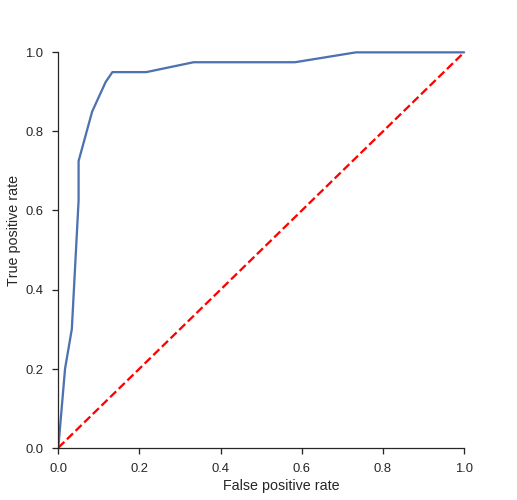
\includegraphics[width=0.7\textwidth]{images/assignment4_3.png}
    \caption{ROC curve resulting from varying the $b$ parameter in the model from Point 1.}
    \label{fig:assignment4_3}
\end{figure}

\section*{Assignment 5}

The biggest point of improvement would be the iteration over the samples, in line 5.
If the block of lines 5-15 could be expressed as matrix operations, one could take advantage of the optimizations of linear algebra libraries.

\section*{Assignment 6}

For this assignment, three rounds of cross validated grid search were performed, one for each pair of classes.
In all cases only the linear kernel was used, the $C$ parameter was explored in the logarithmic range $[1E^0, 1E^4]$ and
the kernel's $r$ parameter \footnote{Linear kernel's definition: $k(x, y) = \langle x, y \rangle + r$} was explored in the linear range $[-10, 10]$.

The best parameters found, together with their minimum losses, are listed in \tabref{table1}:

\begin{table}
    \centering
    \begin{tabular*}{0.61\textwidth}{|l|l|l|l|}
        \hline
        Classes & Test Loss        & $C$ & $r$ \\
        \hline
        1 vs 2  & $= 0$            & 1                  & $\approx -7.1429$   \\
        1 vs 3  & $= 0$            & 1                  & $\approx -7.1429$   \\
        2 vs 3  & $\approx 0.3333$ & $\approx 3.7275$   & $\approx 1.4286$   \\
        \hline
    \end{tabular*}
    \caption{Iris dataset experiment's results}
    \label{tab:table1}
\end{table}

\section*{Assignment 7}

\subsection*{Point 1.}

\begin{table}
    \centering
    \begin{tabular*}{0.544\textwidth}{|l|l|}
        \hline
        kernel     & definition \\
        \hline
        linear     & $k(x, y) = \langle x, y \rangle$ \\
        polynomial & $k(x, y) = (\gamma\langle x, y \rangle + r)^d$ \\
        Gaussian   & $k(x, y) = \exp(-\gamma \Vert x, y\Vert^2_2)$ \\
        \hline
    \end{tabular*}
    \caption{Kernel's definitions}
    \label{tab:table2}
\end{table}

For this assignment, nine rounds of cross validated grid search were performed. In each round one digit was chosen as the positive class, and the rest were set as the negative class.

In all cases linear, polynomial and Gaussian kernels were tried. The definition of each kernel is shown in \tabref{table2}

The $C$ parameter was explored in the logarithmic range $[1E^0, 1E^4]$. This was the only hyperparameter explored for linear kernels.

For polynomial kernels, the $degree$, $\gamma$ and $r$ hyperparameters were also explored in the values $[1, 2, 3]$, logarithmic range $[-1, 2]$ and values $[-2, -1, 0, 1, 2]$, respectively.

For Gaussian kernels, the $\gamma$ hyperparameter was also explored in the logarithmic range $[-1, 2]$.


The best parameters found, together with their minimum losses, are listed in \tabref{table3}:

\begin{table}
    \centering
    \begin{tabular*}{0.775\textwidth}{|l|l|l|l|l|l|l|}
        \hline
        Digit & Kernel     & Test Loss        & $C$ & $\gamma$ & $r$ & $degree$ \\
        \hline
        0     & polynomial & $\approx 0.002$  & 1   & 0.1      & 1   & 2        \\
        1     & polynomial & $\approx 0.002$  & 10  & 0.1      & 2   & 2        \\
        2     & polynomial & $\approx 0.0261$ & 1   & 1        & 2   & 3        \\
        3     & polynomial & $\approx 0.0221$ & 1   & 0.1      & 2   & 3        \\
        4     & polynomial & $\approx 0.0201$ & 1   & 0.1      & 1   & 2        \\
        5     & polynomial & $\approx 0.0261$ & 1   & 10       & 2   & 2        \\
        6     & polynomial & $\approx 0.004$  & 1   & 0.1      & 1   & 3        \\
        7     & polynomial & $\approx 0.0141$ & 1   & 1        & 1   & 3        \\
        8     & polynomial & $\approx 0.0141$ & 1   & 10       & 2   & 2        \\
        9     & Gaussian   & $\approx 0.0141$ & 10  & 0.1      & NA  & NA       \\
        \hline
    \end{tabular*}
    \caption{USPS experiment's 1-vs-rest results}
    \label{tab:table3}
\end{table}

\subsection*{Point 2.}

\Figref{assignment7_2} shows, for each digit, five randomly selected support vectors, together with five randomly selected images from the training set, with the same label.

\begin{figure}
    \centering
    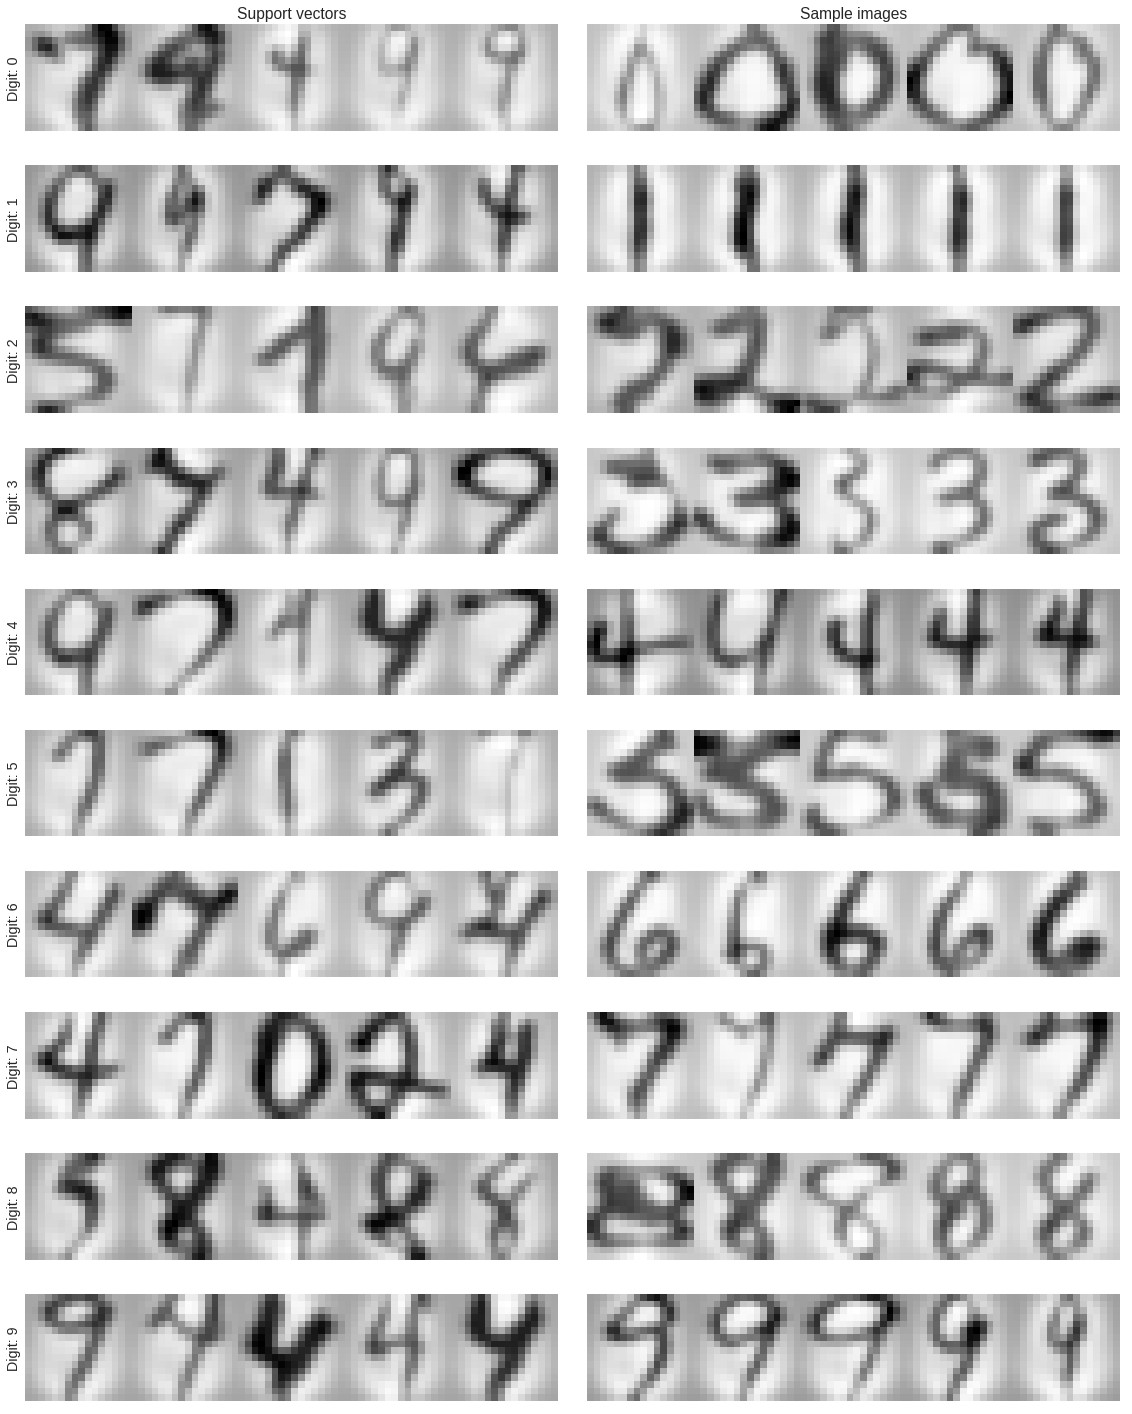
\includegraphics[width=\textwidth]{images/assignment7_2.png}
    \caption{USPS experiment - sample support vectors (right) and sample images(left). Each row indicates which digit was used as the positive class.}
    \label{fig:assignment7_2}
\end{figure}

\subsection*{Point 3.}

A problem could arise from class imbalance.
Given that there are much more negative examples in the one-vs-rest setting, misclassified positive examples end up contributing little to the overall loss.
One possible solution could be to weight an individual sample's error proportionally to the inverse of the sample's class frequency.

\end{document}

